\chapter{Design and Solution}

\section{System Structure}

Overall, the whole system includes three parts of hardware modules, naming camera module, user's smartphone, and the server.

Our sign language translating AI system includes six main modules: hand pattern recognition, direction determination, location detection, action detection, word decoder, and text to speech (Figure 4). Firstly, the system continuously captures the hand’s motion, processes it with the hand landmark model, and then puts it into those modules. Each of them has a unique role, and after combining the first four modules’ results (hand pattern, direction, location, and action detection), the word decoder module will take the output data and bring out the corresponding result. Then, the result will show up on the main screen (Figure 16); meanwhile, the phone will speak out that word. In the below sections, we will discuss each module’s role and how it works.

TODO: Replace with new structure
TODO: Trình bày cả 2 mô hình, giới thiệu luôn action detection và nói là do không khả thi nên đề xuất mô hình mới, khi đó sẽ có sự thay đổi như thế nào 

\begin{figure}[H]
  \centering
  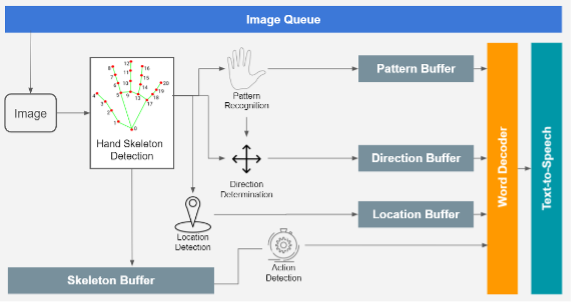
\includegraphics[width=\textwidth]{img/Chap4/OverviewOfTheSystemModules.png}
  \caption{Overview of the system modules}
  \label{fig:Chap4-OverviewOfTheSystemModules}
\end{figure}

\section{Detail Implementation}

\subsection{Hand pattern recognition}

Hand pattern recognition is the first and basic module of this system. While a person with disabilities does signs of sign language, his hands perform a series of different movements, where their hand may be spread out, clenched, or his fingers pointing out at something. Therefore, the role of this module is to recognize the pattern of the hands. Then combining the outcome with other modules, the system can give out the final result.

This module uses the output of the hand landmark model, which is a matrix size of 21. After calculating all the values in that matrix, we get a new matrix representing the distance between those 21 coordinates. Using the distance matrix as the input of CNN [2] with the designed structure (see Figure \ref{fig:Chap4-StructureOfConvolutionalNeuralNetwork}), as seen in Figure \ref{fig:Chap4-OverviewOfTheSystemModules}, will tell us the pattern of the hand at the moment it is captured.

\begin{figure}[H]
  \centering
  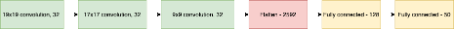
\includegraphics[width=\textwidth]{img/Chap4/StructureOfConvolutionalNeuralNetwork.png}
  \caption{Structure of convolutional neural network}
  \label{fig:Chap4-StructureOfConvolutionalNeuralNetwork}
\end{figure}

\subsection{Direction determination}
FIXME: Thêm các hình ảnh về cách xác định hướng, lấy từ ppt
The directions of the hand include four directions, i.e., right, left, up, down, front, and back. Each hand’s pattern combined with different directions leads to a different meaning. For example, the pattern that points at someone means the word “you”; on the other hand, when we point it to ourselves, it means the word I (see Figure \ref{fig:Chap4-WordYouInSignLanguage} and Figure \ref{fig:Chap4-WordIInSignLanguage}).

\begin{figure}[H]
  \centering
  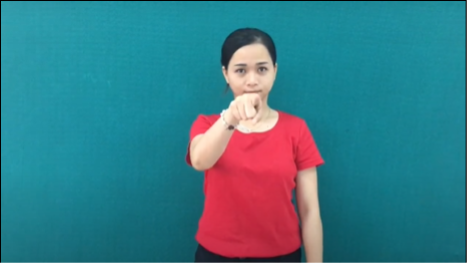
\includegraphics[width=\textwidth]{img/Chap4/WordYouInSignLanguage.png}
  \caption{Word “You” (bạn) in sign language}
  \label{fig:Chap4-WordYouInSignLanguage}
\end{figure}

\begin{figure}[H]
  \centering
  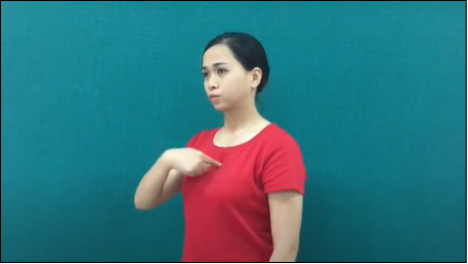
\includegraphics[width=\textwidth]{img/Chap4/WordIInSignLanguage.png}
  \caption{Word “I” (tôi) in sign language}
  \label{fig:Chap4-WordIInSignLanguage}
\end{figure}

To determine the hand’s direction, we use the hand landmark model provided in MediaPipe (see section 2 TK). The inception here is that we calculate the distance between the tip of the index finger and the wrist (called TK), then project it to the axis Ox, Oy, Oz, respectively. After that, we take each of those coordinates and compare them with the others. Finally, the one with the immense value will tell which axis the hand is on; besides, with the direction from the wrist to the tip of the index finger projected on that corresponding axis, we will know which direction the hand is.

For instance, a hand is known to be pointing toward the left direction. The value of the distance, when projected on the axis Ox, will be the biggest one among the three projected values. Then, calculate the vector drawn from the wrist to the tip of the index finger; we will know the direction of the hand itself.

\subsection{Location detection}
FIXME: Giới thiệu previous approach về sử dụng độ zoom, các khó khăn
FIXME: Thêm các hình ảnh về cảm biến sóng âm, các thông số, tại sao lại sử dụng, sử dụng như thế nào

Locations of hand vary, is the hand put at forehead, mouth or the chest level, and so on. Every hand pattern that goes with every location will result in different words. Nevertheless, it is hard for the AI to know the hand’s location with only one camera, and its view is from above (see Figure \ref{fig:Chap4-ViewFromCamera}). However, we came up with some solutions to this issue.

Firstly, we will take pictures of the hand and calculate the size of the hand in every frame in order to know whether that hand is getting bigger or smaller. Hence, if that hand is smaller than before, it means the hand is getting far away from the camera, and its location is somewhere at the chest level or the stomach level.

\begin{figure}[H]
  \centering
  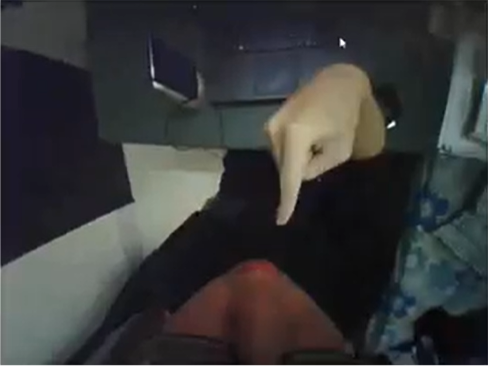
\includegraphics[width=\textwidth]{img/Chap4/ViewFromCamera.png}
  \caption{View from the camera module}
  \label{fig:Chap4-ViewFromCamera}
\end{figure}

Nonetheless, the above solution still has an issue: every man’s hand has a different size, and the system does not know the correct position of the hand. Therefore, another solution is to use a wide-angle camera and set it away from the forehead. With this solution, the camera can have a much broader view. However, since we only have a normal-angle camera, we could not try out this solution and confirm its suitability.

\subsection{ Design}
  TODO: Trình bày các thiết kế hiện có và các chức năng phụ

\subsection{Word decoder}
TODO:   Previous approach 
      [x] How to map word ?
TODO:   New approach
      [x] Punish function
      [x] Using beam search
      [x] CTC decode
      [x] Flow
      [x] Expected result
      [...] Difficult and proposed solution
      [...] Dịch sang tiếng anh
      [...] Thêm các hình ảnh


    TODO: With previous approach

    Như chúng tôi đã trình bày ở phần 1, do có những khó khăn 
    về mặt kĩ thuật trong việc triển khai module
    action detection, chúng tôi đã đề xuất một mô hình mới.
    . Và với mô hình này, module word decode cũng sẽ bị thay đổi
    , nếu như với mô hình cũ, một word sẽ được trình bày dưới dạng
    4 thành phần cơ bản (pattern, location, direction, action),
    khi đó, nhiệm vụ của chúng ta là tìm trong cơ sở dữ liệu, từ nào
    tương ứng với các kết quả thu được từ 4 module trên, khi đó
    ta sẽ thu được từ vựng.

    TODO: Insert image represent the way to map word with 4 module
                              [p,l,d,a]
                        Map   [p1,l1,d1,a1]
              [p,l,d,a] ----> [p2,l2,d2,a2] ---> word
                              [p3,l3,d3,a3]
              Input             database

    Hình trên cho chúng ta thấy cách map một từ vựng sẽ như thế nào.
    Bằng việc so trùng các ký tự, ta sẽ tim được từ vựng phù hợp.
    Nếu không tìm thấy, chúng ta sẽ loại bỏ nó và lấy một bộ khác
    để giải mã.
    Sau khi map được từ vựng, chúng ta sẽ xuất từ vựng đó lên màn hình
    \subsubsection{ Introduction to handstate }
      TODO: Dịch sang tiếng anh
      Lúc này, khi module action detection đã bị lược bỏ. Câu hỏi được đặt ra là,
      làm cách nào để chúng ta có thể không dùng module action detection nhưng vẫn có thể
      nhận diện được từ vựng
      Do đó, nhóm tác giả đề xuất một mô hình khác cho từ vựng, lúc này
      một từ không còn được cấu thành từ 4 thành phần cơ bản như ở mô hình cũ nữa,
      mà sẽ được cấu thành từ nhiều thành phần khác nhau, mỗi thành phần tương ứng
      sẽ chứa trong nó là một bộ 3 : pattern, direction, location. Tương ứng với mỗi
      bộ 3 này, chúng tôi sẽ gọi nó là một hand_state và như thế, ta có thể hiểu một từ vựng
      sẽ được cấu thành từ nhiều hand_state khác nhau. Ý tưởng của vấn đề xuất phát
      từ các nghiên cứu của xử lý ngôn ngữ tự nhiên, khi một từ sẽ được cấu thành từ
      nhiều ký tự, thì trong trường hợp này, một từ sẽ được ghép từ nhiều hand_state.
      Sau đó, khi qua các bước xử lý mà chúng tôi sẽ trình bày ở bước sau, ta sẽ thu được từ vựng mong muốn
      FIXME:Insert image from ppt about hand_state

    \subsubsection{ Using beam search and CTC decode to map word }
      Sau khi chúng ta đã nắm được khái niệm về hand_state, chúng ta sẽ đi đến phần quan trọng
      nhất của mô hình: chuyển đổi các hand_state đã nhận được thành từ vựng.
      
      # Insert image about : mô hình như thế nào (lấy từ ppt)

      Fig ... là mô hình mà nhóm tác giả đề xuất cho phần này. Input đầu vào
      sẽ là một hàng đợi các hand_state được lấy từ 3 component trước đó. Ở đây nhóm tác giả
      quy ước chiều dài của hàng đợi là 5, tuy nhiên cần có sự tính toán và thử nghiệm để tìm
      được độ dài hàng đợi phù hợp.
      Mô hình này gồm ... bước:
        + Vectorization: Đây là bước chuyển đổi từ một hàng đợi gồm nhiều hand_state thành
        một ma trận làm input đầu vào cho beam search
        + Beam search : Ở bước này, chúng ta sẽ thực hiện giải thuật beam search để chọn ra
        từ cơ sở dữ liệu các hand_state nào là phù hợp với input đưa vào. Bên cạnh đó, ở bước
        này, nhóm tác giả đề xuất sử dụng mô hình CTC decde để có thể loại bỏ những hand_state bị sai
        hoặc những hand_state bị trùng lặp trước đó, tăng tính hiệu quả cho mô hình.
        + Map to dictionary: Và cuối cùng, sau khi qua 2 bước trên, từ hàng đợi ban đầu, ta sẽ
        thu được các hand_state có khả năng nhất. Việc cần làm của chúng ta là map các hand_state
        này vào cơ sở dữ liệu và tìm ra từ vựng phù hợp.
      
    \subsubsection{ Vectorization }
      TODO: Why we need punish
      TODO: how to perform -> Trình bày cách đánh giá như thế nào, cách trừ điểm và các phương châm đánh giá
      TODO: Sau khi punish dùng hàm softmax để chuyển các giá trị về dạng xác suất

      Khi đến bước này, những gì chúng ta nhận được sẽ là: một hàng đợi của các hand_state.
      Do trước khi vào module beam search, ta cần một matrix biểu diễn sự tương quan giữa các output nhận được từ các component và các dữ liệu trong database
      # Insert image about hand_state queue
      Từ hàng đợi này, ta sẽ lấy lần luọt từng hand_state, so sánh nó với cơ sở dữ liệu về hand_state có sẵn 
      và đánh giá điểm số cho nó dựa trên các nguyên tắc sau:
        + Các hand_state được lấy ra từ hàng đợi nếu có điểm tương đồng càng lớn với một hand_state
        trong cơ sở dữ liệu thì sẽ được đánh giá điểm số càng cao. Ví dụ trong cơ sở dữ liệu chúng ta
        có một hand_state như sau : [p_1, l_1, d_1] và hand_state ta nhận được từ input là [p_1, l_1, d_1] thì hand_state này sẽ
        được đánh giá điểm số cao hơn hand_state [p_1, l_1, d_2]. Và cứ như thế, ta sẽ lần lượt cho điểm các hand_state lấy ra từ hàng đợi
        + Khi đánh giá các hand_state, đối với trường hợp so trùng 2 pattern. Do các pattern này được nhận diện từ module
        hand pattern regconition (vision approach), do đó, sẽ có khả năng bị nhận diện bị sai, hoặc bị nhầm. Vì lẽ đó, để có thể
        đánh giá một cách chính xác và công bằng nhất có thể thì ở đây, đối với những pattern hay bị nhận diện sai, ta sẽ trừ điểm thấp và ngược lại
        , với những pattern đơn giản mà hệ thống lại nhận diện sai thì sẽ bị trừ điểm nhiều hơn
      
      Sau khi hoàn thành bước đánh giá và cho điểm như trên, ta sẽ dùng một hàm để normalize
      lại dữ liệu (ở đây nhóm tác giả sử dụng softmax function) và trả về cho chúng ta một bộ xác suất của các hand_state trong hàng đợi. Ta sẽ sử dụng bộ xác suất này
      làm input đầu vào cho bước beam_search.
    \subsubsection{ Using beamsearch with CTC decode }
      TODO: Trình bày cách sử dụng beamsearch để tìm các cặp bộ 3
      TODO: Image beamsearch (get from ppt)
      TODO: Example
      TODO: Áp dụng CTC để handle một số trường hợp
      TODO: Các khó khăn gặp phải và hướng giải quyết
      
      Sau khi qua bước vectorizaion, các hand_state trong hàng đợi của chúng ta
      đã được chuyển đổi thành một ma trận MxN với M là độ dài của cơ sở dữ liệu về
      các hand_state và N là độ dài của hàng đợi.
      
      Bằng việc sử dụng beam search, từ sẽ thu được k hand_state có khả năng nhất
      từ cơ sở dữ liệu. Từ hình ảnh bên dưới, ta có thể hình dung được những gì
      đã diễn ra sau trong quá trình thực hiện beam search
      FIXME: Insert image from ppt about matrix with beam search

      Tuy nhiên, có thể thấy được rằng, sau khi thực hiện xong bước beamsearch,
      ta sẽ thu được một dãy các hand_state có độ dài tương ứng với độ dài của hàng đợi
      , các hand_state này có thể bao gồm những hand_state bị trùng nhau, hoặc cũng có thể
      là những hand_state bị sai. Do đó, ta cần áp dụng thêm CTC decode để loại bỏ các hand_state
      bị trùng này. Đối với những hand_state bị nhận sai từ những module trước thì ở bước Vectorization,
      ta sẽ đặt một threshold để loại bỏ những hand_state này và xem như hand_state đó là một ký tự rỗng ("_")
      và cuối cùng, sau khi áp dụng CTC decode vào, ta sẽ thu được kết quả mong muốn

      FIXME: Insert image about the result (get from ppt)

      
      
    \subsubsection{ Map to dictionary }
      TODO: Cách map như thế nào
      Sau khi nhận được một tập các hand_state có khả năng nhất, việc còn lại là
      chúng ta sẽ map vào cơ sở dữ liệu, như cách mà chúng ta đã làm trong mục ..., 
      nhưng thay vì map với bộ 4 thành phần thì ở đây, ta sẽ map với input các hand_state thu được
      từ bước ... .
      Và như thế, ta sẽ thu được từ vựng mà không cần phải dùng tới module action detection.

\subsection{Text to speech}

Besides displaying the translated sign language in text form, we included a text-to-speech module to know the result without looking into the screen. This module makes use of a free API provided by Google, named Text-to-Speech [4]. It converts arbitrary strings, words, and sentences into the sound of a person speaking the same things.
